\subsection{Beleuchtung}
\label{subsec:Inbetriebnahme_Beleuchtung}

Die Farbe und Helligkeit der Beleuchtung wird mit einem PWM-Signal geregelt. Das PWM-Signal wird erzeugt mittels Timer Interrupts, damit Regelung parallel neben dem Programfluss geschehen kann. Insgesamt benötigt es fünf Timer, um das LED-Band anzusteuern. Jeweils einen für jede Farbe und einen um durch den Rainbow-Modus zu interieren.

\subsubsection{PWM-Signale LED}

Das PWM-Signal für die LEDs wird mit einer Frequenz von 10 kHz initialisiert. Um dies zu erreichen, wird Formel \ref{equ:Timer_Max_1} umgestellt nach \ref{equ:Timer_Max_2}. Der Prescaler ist N = 1. Das Ergebnis wird im Register OCRnA gespeichert, wodurch der Timer $1/10kHz = 100\mu s$ benötigt, bis ein Timer\_nx Compare-Interrupt ausgelöst wird.

\begin{equation}
f_{OC_{max}} = \frac{f_{clk_{I/O}}}{2 \cdot N \cdot (1+OCR_{nA})}
\label{equ:Timer_Max_1}
\end{equation}

umgestellt nach OCR\_nx:

\begin{equation}
OCR_{nx} = \frac{f_{clk_{I/O}}}{2 \cdot N \cdot f_{OC_{max}}} - 1 = \frac{16MHz}{2 \cdot 1 \cdot 10kHz} - 1 = 799
\label{equ:Timer_Max_2}
\end{equation}

Damit das Hochzählen des Counters nach erreichen von OCRnA wieder bei null beginnt, wird der Timer im CTC-Mode betrieben. Das Register OCRnA stellt so den maximalen Wert des Counters dar. Dies ist in Abbildung \ref {fig:Timer_CTC_Mode} und \ref{fig:Timer_CTC_Timing_Diagram} zu sehen.

\begin{figure}[h!]
	\centering
	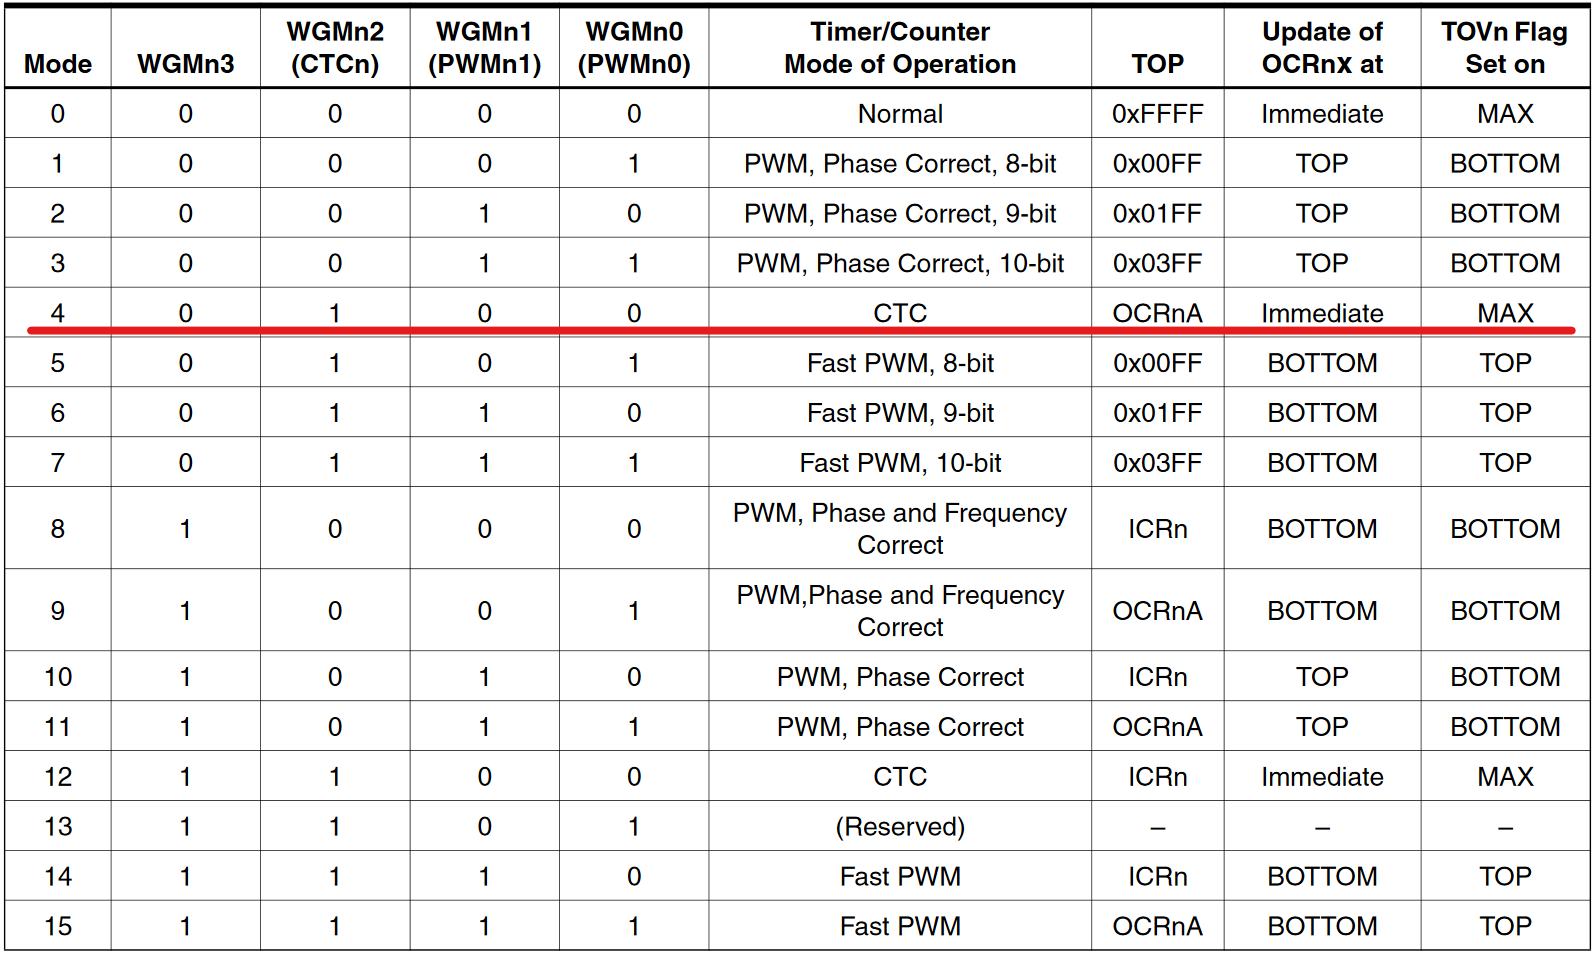
\includegraphics[width=\textwidth]{graphics/Timer_CTC_Mode}
	\caption{Timing-Diagramm CTC-Mode. OCnx nicht angeschlossen, Pin wird softwaremässig getoggelt.}
	\label{fig:Timer_CTC_Mode}
\end{figure}

\begin{figure}[h!]
	\centering
	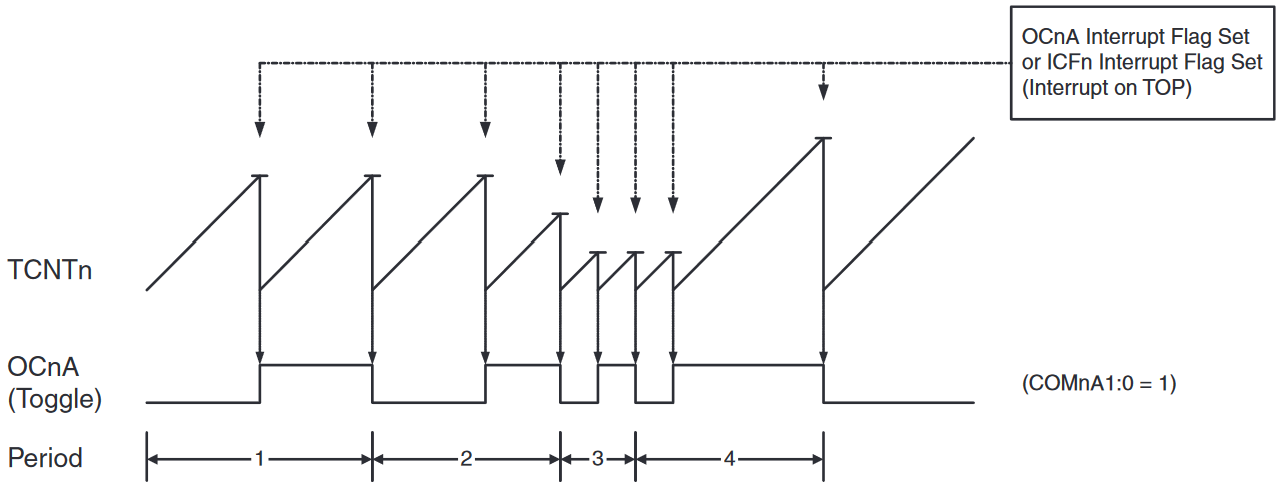
\includegraphics[width=\textwidth]{graphics/Timer_CTC_Timing_Diagram}
	\caption{Timing-Diagramm CTC-Mode. OCnx nicht angeschlossen, Pin wird softwaremässig getoggelt.}
	\label{fig:Timer_CTC_Timing_Diagram}
\end{figure}

\todo{cites: Atmel Datenblatt S.146}

Der Duty-Cycle wird Prozentual zum OCRnA-Register gesetzt. Wird für den berechneten Wert ein Duty-Cycle von 50\% vorgegeben, ergibt sich für das OCRnB-Register den Wert $(800 / 2) -1 \approx 399$. So wird nach der Hälfte der Hochzählzeit ein zweiter Compare-Interrupt ausgelöst, welcher jedoch kein Einfluss auf das Counter-Register hat.

Nun muss in beiden der erwähnten Interrupt-Routinen das gewünschte LED getoggelt werden. In der ersten Interruptroutine mit dem OCRnA-Compare-Register wird die LED eingeschaltet, in der zweiten Interruptroutine mit dem OCRnB-Compare-Register wird die LED ausgeschaltet.

Möchte man nun die Helligkeit angepasst werden, kann ein Wert zwischen 0 und OCRnA ausgewählt werden und damit das Register OCRnB beschrieben werden.

\todo{cite:  Formel - Atmega datenblatt S.121 }
\todo{cite:  Prescaler - Atmega datenblatt S.129 }
\todo{cite:  CTC-Mode - Atmega datenblatt S.145 }
\todo{cite:  CTC-Timing-Diagramm - Atmega datenblatt S.146 }

Der Wert für das OCRnA-Register ist folglich 799. Ein OCRnB-Register wird nicht benötigt, da die Iteration nur ausgeführt wird, sobald ein OCRnA-Compara-Match-Interrupt ausgelöst wird.

\subsubsection{Custom-Funktion}

Bei der Custom-Funktion können die Farbwerte manuell definiert werden. So wird für eine bestimmte Farbe für jede LED-Farbe der entsprechende Wert in das OCRnB-Register geschrieben. Darf sich eine Farbe nicht verändern, so muss das OCRnB-Register den gleichen Wert behalten. Die Itearation durch den Rainbow-Algorithmus wird im Custom-Mode nicht benötigt.

\subsubsection{Rainbow-Funktion}

Die Farbe der RGB-LED soll nun jeweils fünf Sekunden brauchen, um einen Farbteil komplett ein- oder auszuschalten, was einen sanften Übergang im Farbkreis ermöglicht.

Im Rainbow-Loop gibt es sechs States. Zubeginn muss die grüne LED schon voll leuchten.
\begin{enumerate}
\item Start ==> Grün
\item Hochzählen des Rot-Anteils ==> Yellow
\item Runterzählen des Grün-Anteils ==> Rot
\item Hochzählen des Blau-Anteils ==> Magenta
\item Runterzählen des Rot-Anteils ==> Blau
\item Hochzählen des Grün-Anteils ==> Cyan
\item Runterzählen des Blau-Anteils ==> Grün
\item Repeat 2 - 7
\end{enumerate}

Es benötigt 800 Schritte um einen Farbteil komplett ein- und auszuschalten. Pro Interrupt wird ein Schritt hochgezählt. Mit Formel \ref{equ:Milli_S} kann direkt berechnet werden, mit welchem Wert das Compare-Register beschrieben werden muss, sodass es fünf Sekunden geht, bis 800 Schritte hochgezählt wurden.

\begin{equation}
OCR_{nx} = \frac{f_{clk_{I/O}}}{2 \cdot N \cdot f_{OC_{max}}} - 1 = \frac{16MHz}{2 \cdot 1024 \cdot \frac{5s}{800 Schritte}} - 1 \approx 48
\label{equ:Milli_S}
\end{equation}

Die Iteration durch den Rainbow-Modus wird folglich mit einer Frequenz von 160Hz initialisiert. In der Routine wird demnach alle 6.25ms der Duty-Cytle einer Farbe hoch oder runtergezählt, und das Timer-Compare-Register des entsprechenden LED-Timers angepasst.

\subsubsection{Vorgehen}

\begin{enumerate}
\item Benötigte Applikation aus dem Software-Ordner auf dem USB-Stick in Atmel Studio öffnen.\\
\textcolor{magenta}{Software\textrightarrow Atmega\textrightarrow 3\underline{ }LED\underline{ }Control\textrightarrow 1\underline{ }LED\underline{ }Testsoftware\textrightarrow LED}\\

\item Software hochladen:\\
\textcolor{blue}{AtmelStudio\textrightarrow Tools\textrightarrow Cocktailmixer}\\

\end{enumerate}